\chapter{Interpretation of morphogen gradients by a bistable circuit}
\label{chapter:double-exclusive}
\epigraph{\textit{memory of younger days}}{Ocarina of Time}
\section{Preface}

\begin{enumerate}
    \item Keep focus on developmental biology
    \item Revised supplement as this chapter
\end{enumerate}

\usetikzlibrary{patterns}
\begin{Figure}
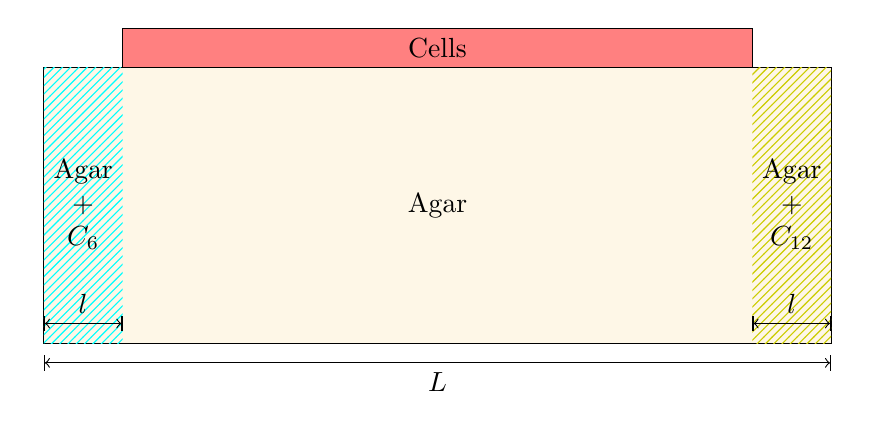
\begin{tikzpicture}
\def\H{3.5}
\def\L{10.0}
\def\l{1.0}
\def\epsilon{0.5}
\def\dx{0.25}
\def\dy{0.25}

%cell region
\filldraw[fill=Red!50!white] (\l,\H) rectangle (\L-\l,\H+\epsilon) node[midway] {Cells};

%agar region
\filldraw[fill=Dandelion!10!white,draw=black] (0,0) rectangle (\L,\H) node[midway] {Agar};
\fill[pattern=north east lines, pattern color=cyan] (0,0) rectangle (\l,\H) node[midway] {\begin{tabular}{c}Agar\\+\\$C_6$\end{tabular}};
\fill[pattern=north east lines, pattern color=yellow!80!black] (\L-\l,0) rectangle (\L,\H) node[midway] {\begin{tabular}{c}Agar\\+\\$C_{12}$\end{tabular}};
\draw[|<->|](0,-\dy) -- (\L,-\dy) node[midway, below] {$L$} ;
\draw[|<->|](0,\dy) -- (\l,\dy) node[midway, above] {$l$} ;
\draw[|<->|](\L-\l,\dy) -- (\L,\dy) node[midway, above] {$l$} ;
%\draw[|<->|](\L+\dx,0) -- (\L+\dx,\H) node[midway, right] {$H$} ;
%\draw[|<->|](\L+\dx,\H) -- (\L+\dx,\H+\epsilon) node[midway, right] {$H_\varepsilon$} ;

%axis
%\draw[->] (-\dx-\dy,-\dy)--(0.1*\L,-\dy) node[right] {$x$};
%\draw[->] (-\dx,-\dx-\dy)--(-\dx,0.5*\H) node[above] {$y$};
\end{tikzpicture}
\caption{Geometry of opposing gradients experiment}
\label{fig:experiment_geometry}
\end{Figure}

This section outlines how the Design---Learn pipeline may help achieve a specific
aim in a typical collaboration between theory, computation and experiment.
The aim of this project is to reconstitute and control minimal self-organisation
mechanisms which are believed play crucial roles in developmental biology. To this
end \textit{E. Coli} has been genetically engineered to produce orthogonal responses
to two different input signals --- henceforth this organism will be referred to as the
\textit{double exclusive reporter} circuit \cite{Grant2016}. The colony of reporters
serve as a reduced model for a multi-cellular organism during embryonic stages of
development. While patterns with sharp boundaries have successfully been realised,
producing Turing instabilities remains challenging as the system needs to be such
that patterns develop before the colony reaches stationary phase.
The role of theory and computation in this project is to help identify the
parameter regimes that produce controllable and self-organised patterns.

\subsection{Developmental Context}
During the development of any organism a hierarchy of self-organisation takes place that leads
to the breaking of symmetry from a spherical cluster of undifferentiated cells to the formation
of organ segments and limbs. This process is known as morphogenesis. figure \ref{fig:morph}
shows an example in which \textit{Hox} gene expression patterns in the body segments of
Drosophila can drastically affect its development.

\begin{Figure}
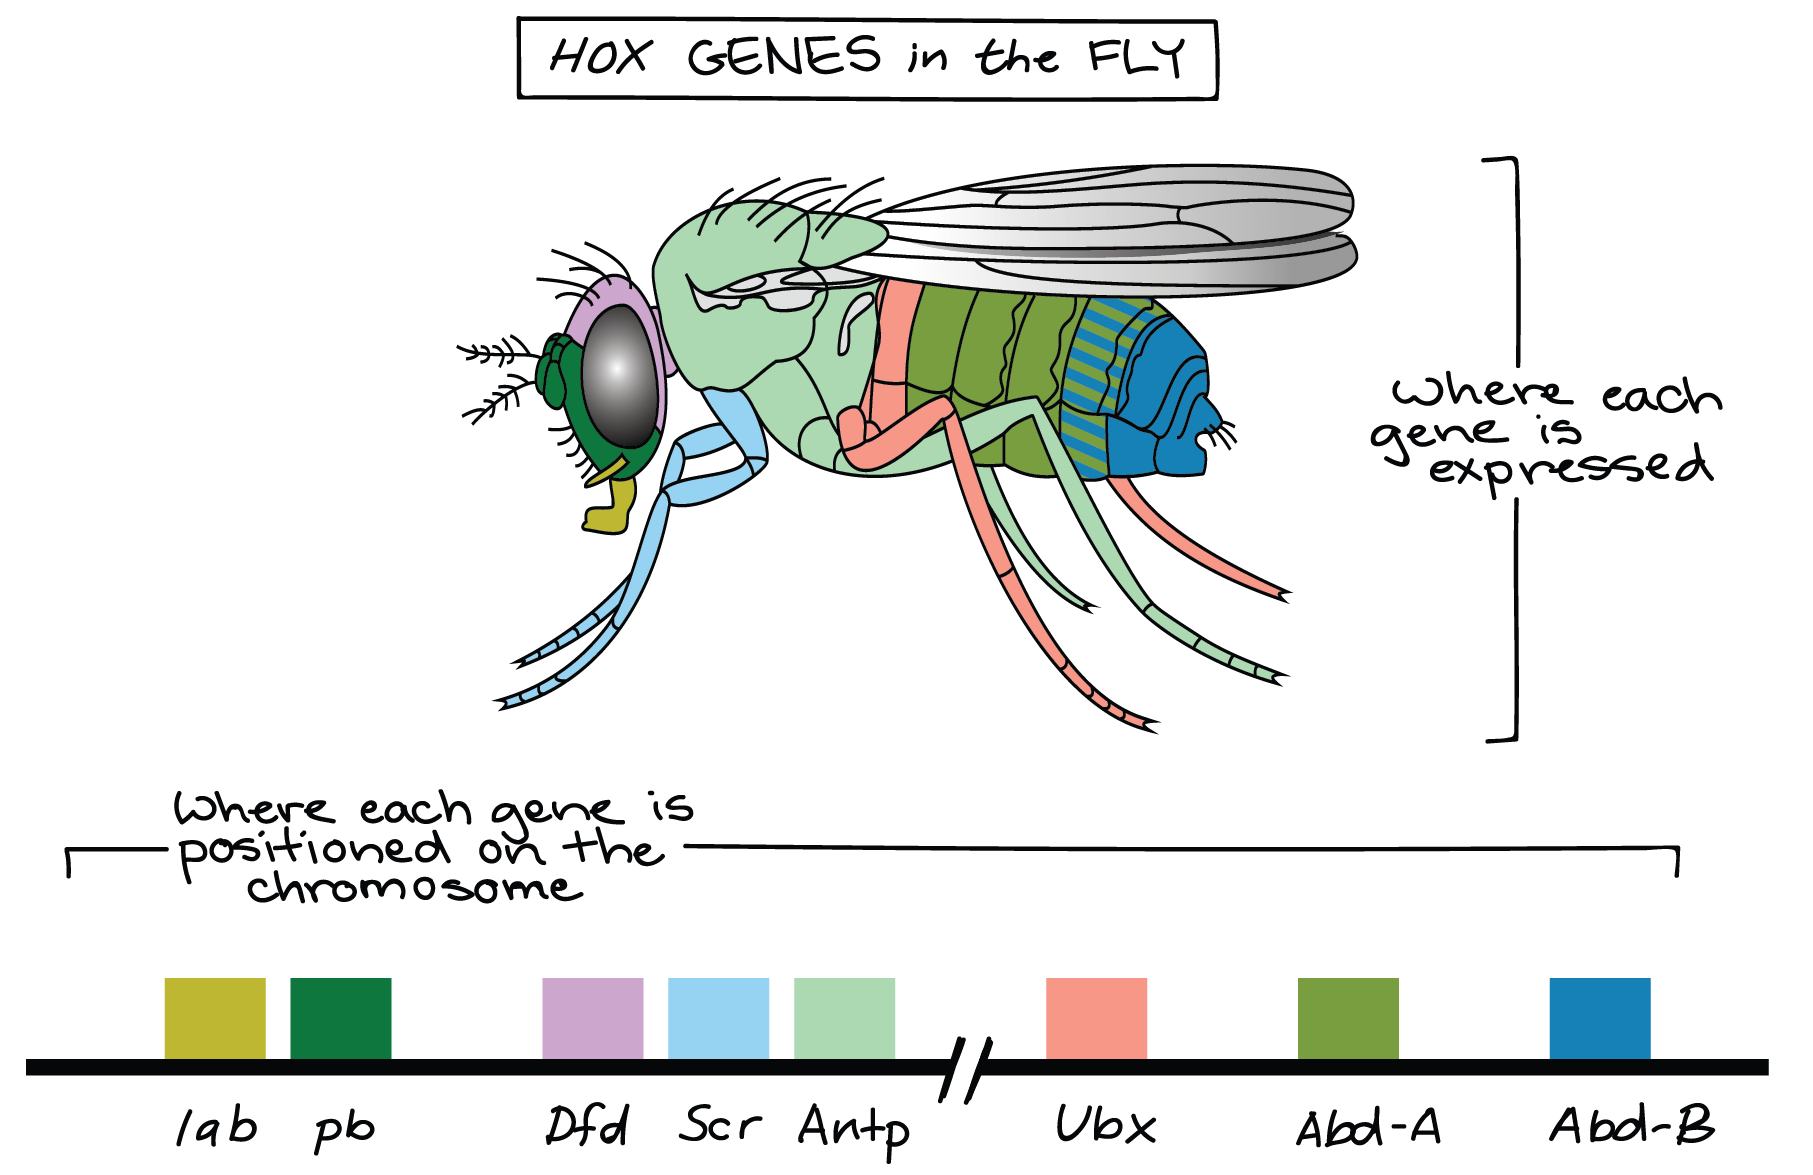
\includegraphics[width=90mm]{figures/morph1.png}\\
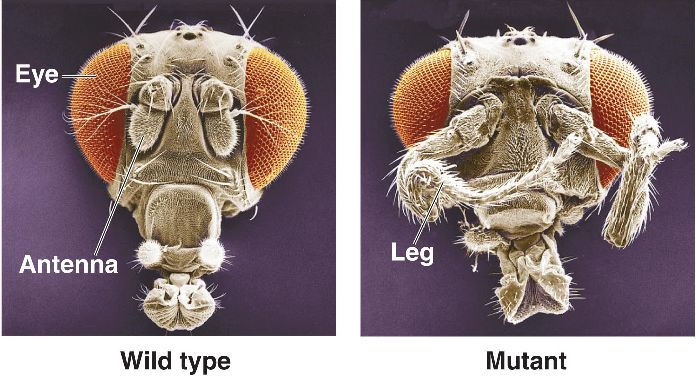
\includegraphics[width=90mm]{figures/morph2.png}
\caption{Top: \textit{Hox} gene expression patterns in body segments of drosophila.\\
Bottom: Mutation where legs grow in-place of antenna}
\label{fig:morph}
\end{Figure}
\subsection{Morphogen-driven Patterns}
One of the central questions in developmental biology is how positional information is
sensed by a population of cells and how sharp gene expression boundaries between
populations are maintained for robust organ and body segment development. The
French Flag model \cite{Wolpert1969PositionalDifferentiation.} proposes that cells
have a threshold response to external signalling molecules -- henceforth referred
to as morphogens -- which pre-pattern the organism from anterior to posterior and
laterally. Some examples of morphogens include Wingless, Decapentaplegic and Sonic Hedgehog.
figure \ref{fig:gap} show the \textit{Gap} expression patterns that partition the
Drosophila embryo into segments which are later differentiated by \textit{Hox} genes.

\begin{Figure}
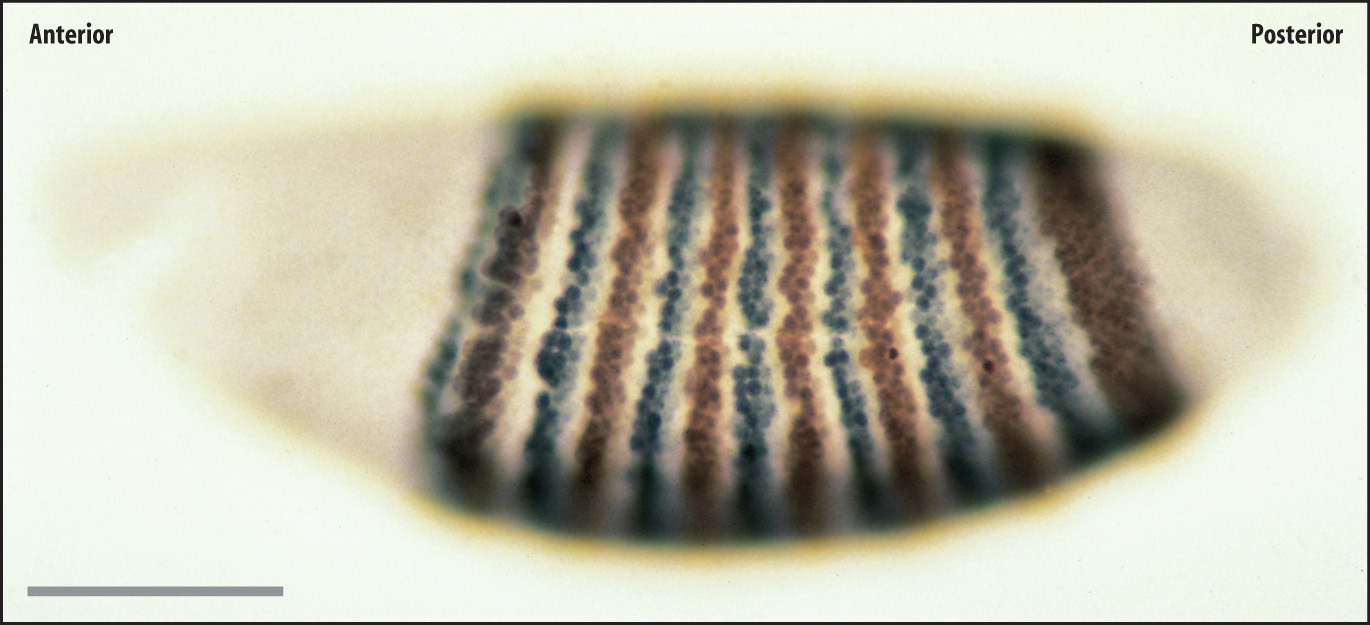
\includegraphics[width=90mm]{figures/gap.jpg}
\caption{Expression patterns of pair-rule \textit{Gap} genes in Drosophila embryo \cite{}}
\label{fig:gap}
\end{Figure}

\subsection{Self-organised Patterns}
How are morphogen gradients set up and maintained? How can they be robust against
changes in size and geometry? A canonical example of self-organisation in bacteria
is the quorum sensing system \cite{Miller2002QuorumBacteria}. Each cell secretes a
signalling molecule resulting in the total concentration being proportional to
the population density. This signal induces adaptive responses in metabolic and
mobility in the whole colony. A long standing mathematical hypothesis that
Turing patterns underlie self-organisation in cell populations. Recent literature
suggests both morphogen-driven and Turing patterning mechanisms play a role in development 
\cite{Green2015PositionalCombine}

\begin{Figure}
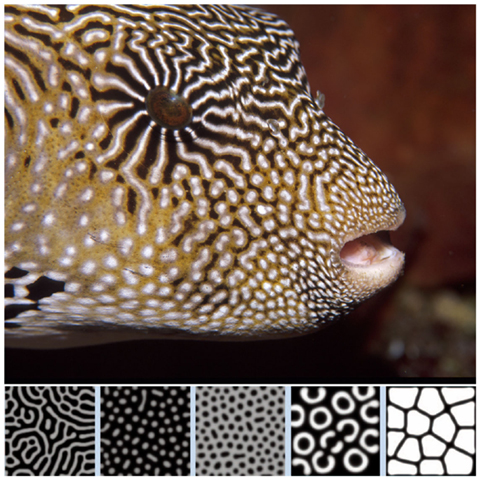
\includegraphics[width=70mm]{figures/turing.png}
\caption{Pigment patterns hypothesised to be generated by Turing mechanism}
\label{fig:turing}
\end{Figure}

\subsection{Learnings \& Limitations}
This section outlines the results on determining the bi-stability landscape for the
\textit{double-exclusive reporter}, and how its geometry helps determine the conditions for
moving and stationary sharp boundary formation. The design of the device is summarised 
in figure \ref{fig:device}. Each wiggly line represents a promoter. Incoming solid lines
to a vertex represents the formation of a complex, which lead to the induction of a promoter.
Outgoing solid lines represent the transcription-translation of genes downstream of a
promoter. Arrows that end in t-junctions represent the repression of a pathway.

\begin{Figure}
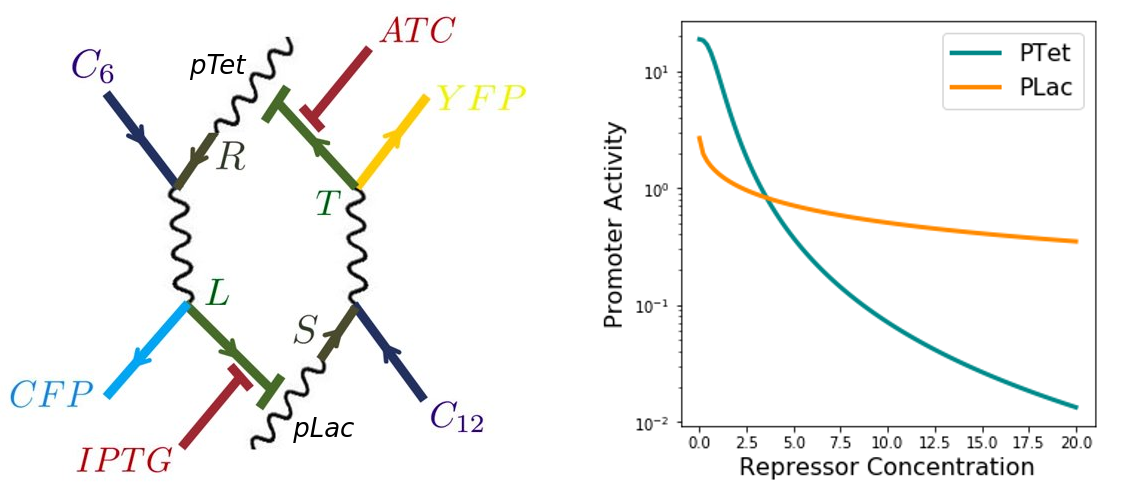
\includegraphics[width=140mm]{figures/device.png}
\caption{Left: Diagram of double exclusive reporter showing wiring between promoters
and complexes Right: Repression of \textit{pTet} and \textit{pLac} promoters via
\textit{TetR} and \textit{LacI} respectively}
\label{fig:device}
\end{Figure}
\noindent
The observable chemicals, labelled \textit{YFP} and \textit{CFP}, are
proportional to their upstream promoter activities. The experimentally controllable chemicals
are quorum sensing molecules $C_6$, $C_{12}$ and de-repressesors \textit{ATC},\textit{IPTG}.
All other chemicals cannot be directly observed. The double-negative feedback loop leads
to bi-stability in the observable signals, which is key to producing sharp gene
expression boundaries.

\begin{Figure}

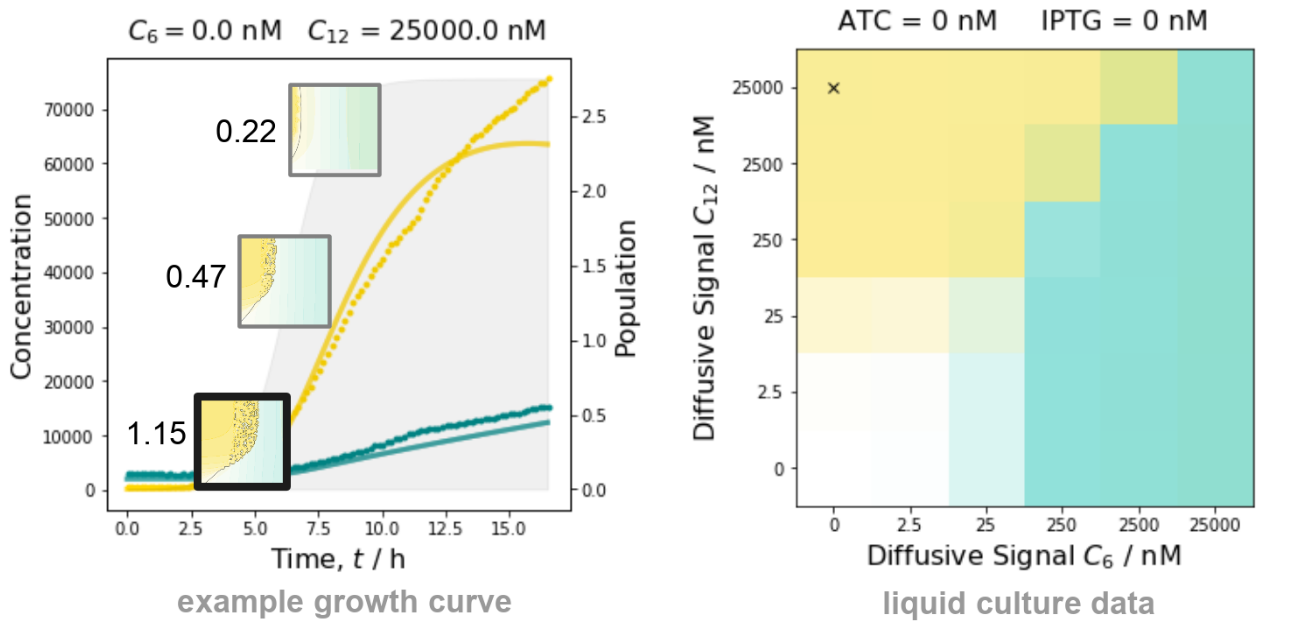
\includegraphics[width=120mm]{figures/microtiter.png}
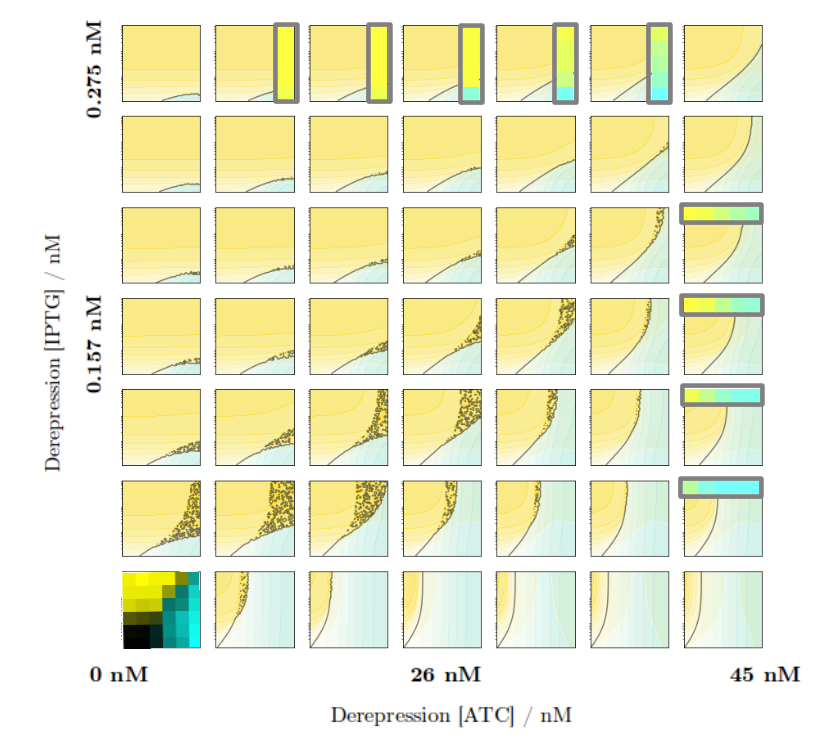
\includegraphics[width=100mm]{figures/parameter-space.png}
\caption{Top Left: Optical density measurements obtained for one well.
Top Right: Final fluorescence values at 16h across different $C_6$, $C_{12}$
concentrations. Bottom: Steady state predictions between data regions.}
\label{fig:microplate-data}
\end{Figure}

\subsection{Microtiter Plate Data}
The synthetic bacterial cultures are grown in suspended media and plated on
96 well microtiter plates in different concentrations of signalling molecules
$C_6$, $C_{12}$ and de-repressesors \textit{ATC},\textit{IPTG}. Then
optical density measurements in \textit{YFP} and \textit{CFP} are taken
from each well every 20min for 16 hours. Cells begin to grow in exponential
phase where the circuit is assumed to function optimally, until the
population eventually reaches stationary phase. figure \ref{fig:microplate-data} across
several different conditions overlayed on top of a model what predicts
the steady state behaviour between collected data regions.

\subsection{Spatial Experiments}
Simulations of the model revealed that if the final homogenous concentrations
of $C_6$ and $C_{12}$ lie within the bistable region, then the prepatterned
signals will form a sharp boundary at their interface. Spatial experiments
shown in figure \ref{fig:boundary} confirm this prediction.
\begin{Figure}
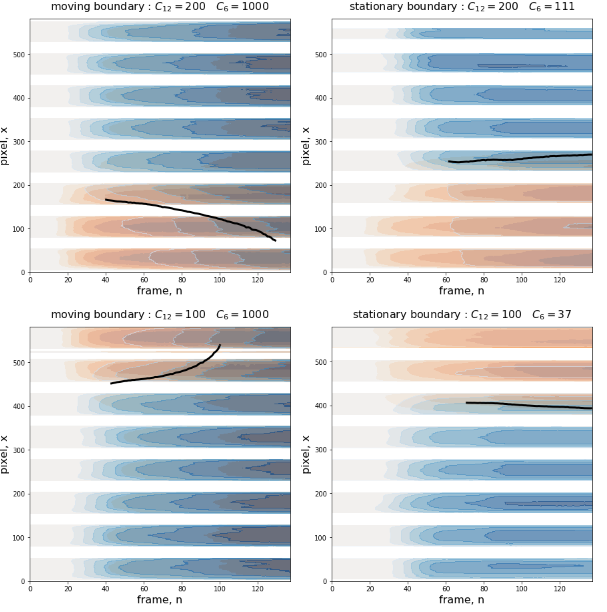
\includegraphics[width=120mm]{figures/spatial.png}
\caption{Merge channel yfp/cfp kymographs showing stationary (right)\\and moving boundaries (left)}
\label{fig:boundary}
\end{Figure}

\subsection{Contributions}
Contributions for this work are as follows


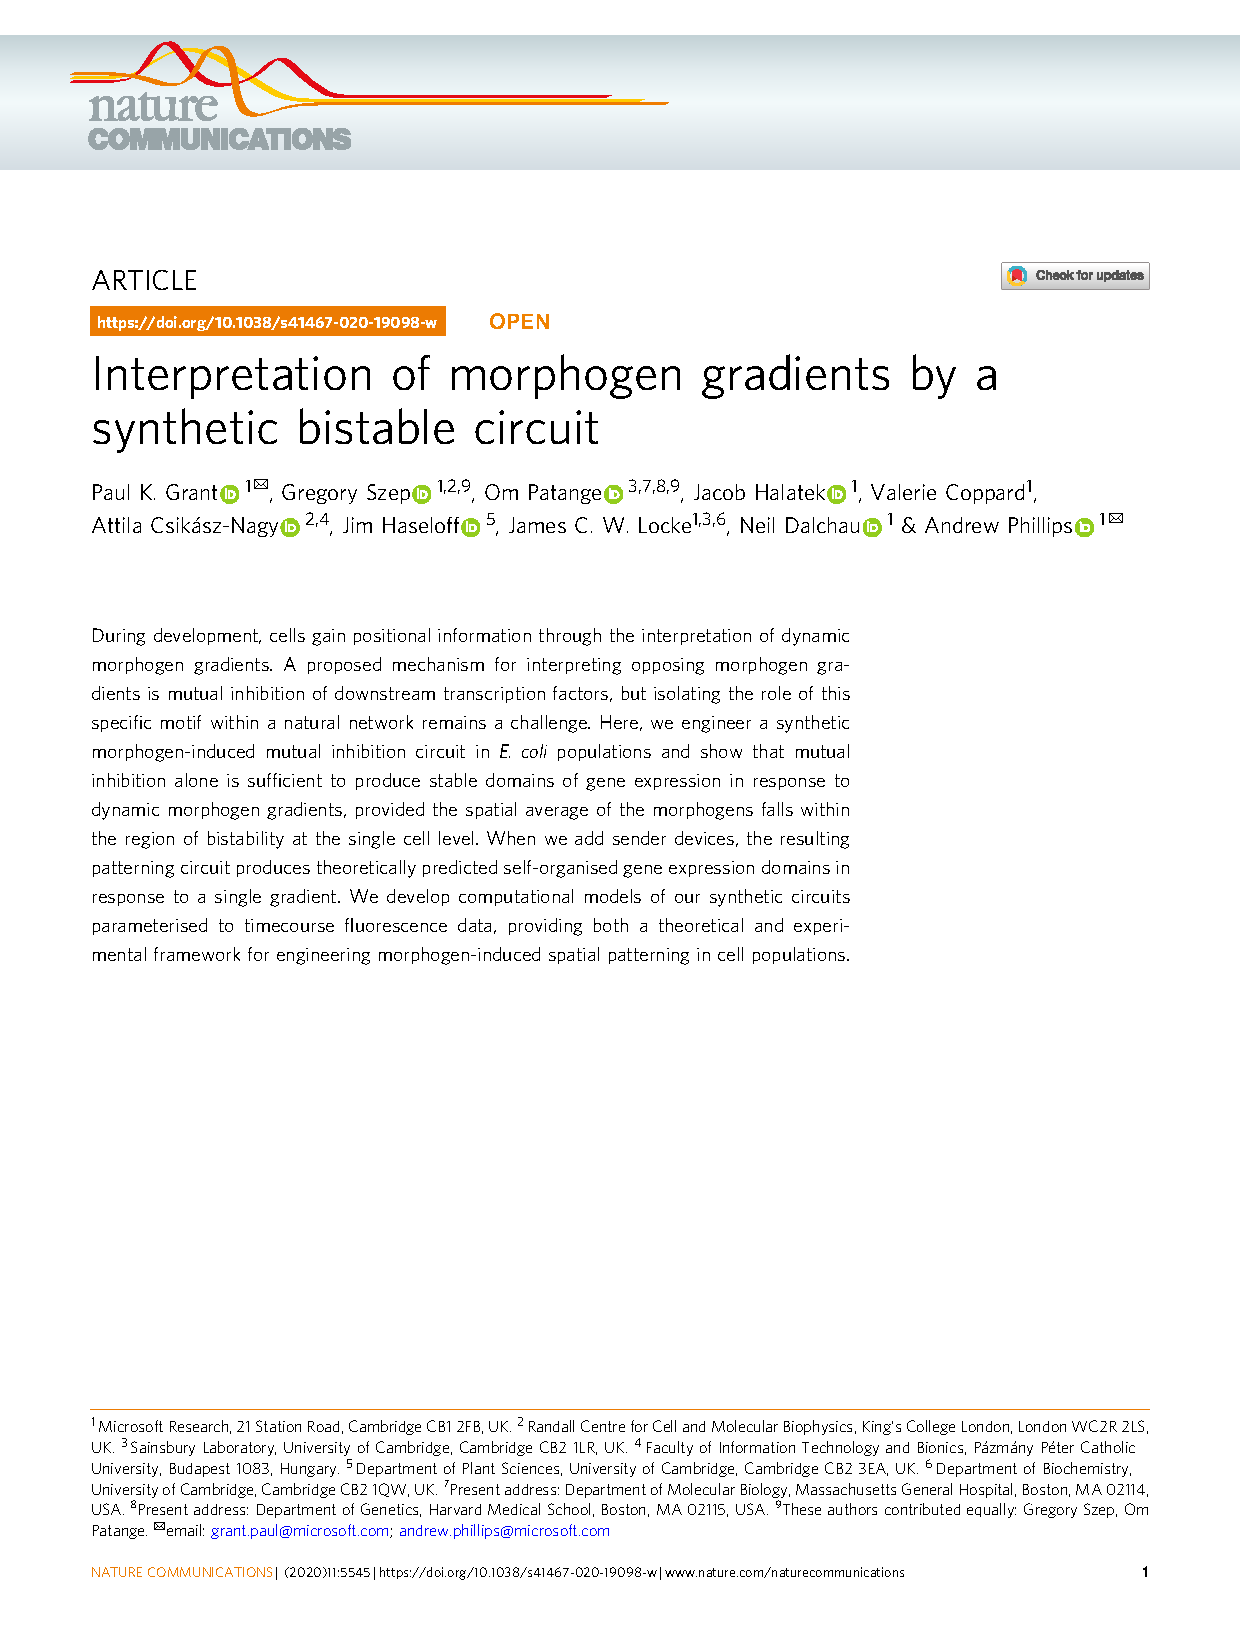
\includepdf[pages=1-8, offset=75 -90, scale=0.85, frame,
        clip,trim=10mm 5mm 10mm 0mm,
        pagecommand={}, addtotoc={
        1,section,1,Abstract,double-exclusive:abstract,
        2,section,1,Introduction,double-exclusive:introduction,
        2,section,1,Results,double-exclusive:results,
        2,subsection,2,Engineering mutual exclusivity,double-exclusive:exclusivity,
        3,subsection,2,Mutual inhibition results in bistability,double-exclusive:bistability,
        4,subsection,2,Hysteresis produces stable boundaries,double-exclusive:boundaries,
        4,subsection,2,A secondary gradient creates self-organised domains,double-exclusive:self-organisation,
        5,section,1,Discussion,double-exclusive:discussion,
        6,section,1,Methods,double-exclusive:methods,
        6,subsection,2,Plasmid construction,double-exclusive:plasmids,
        6,subsection,2,Plate fluorometer assay,double-exclusive:plates,
        6,subsection,2,Flow-cytometric analysis of hysteresis,double-exclusive:flow,
        7,subsection,2,Microfluidics,double-exclusive:microfluidics,
        7,subsection,2,Microfluidics microscopy,double-exclusive:microscopy,
        7,subsection,2,Solid culture assays,double-exclusive:cultures},
    addtolist={
        2, figure, {\textit{Fig. 1}\quad A synthetic gene circuit for morphogen interpretation.}, figure:double-exclusive:overview,
        3, figure, {\textit{Fig. 2}\quad Mutual inhibition produces bistability.}, figure:double-exclusive:bistability,
        5, figure, {\textit{Fig. 3}\quad Formation of stable boundaries.}, figure:double-exclusive:boundaries,
        6, figure, {\textit{Fig. 4}\quad Addition of a Relay circuit creates self-organised domains of gene expression.}, figure:double-exclusive:relay
}]{publications/double-exclusive.pdf}